\documentclass[
reprint,
superscriptaddress,
% groupedaddress,
% unsortedaddress,
% runinaddress,
% frontmatterverbose, 
% preprint,
showpacs,
preprintnumbers,
% nofootinbib,
% nobibnotes,
bibnotes,
amsmath,
amssymb,
aps,
prd,
% onecolumn,
%longbibliography,
%rmp,
%prstab,
%prstper,
floatfix
]{revtex4-2}

\usepackage[utf8]{inputenc}
\usepackage[normalem]{ulem}
\usepackage{graphicx}% Include figure files
\usepackage{dcolumn}% Align table columns on decimal point
\usepackage{bm}% bold math
\usepackage{color}
\usepackage{xcolor}
\usepackage[colorlinks=true,allcolors=purple]{hyperref}
\usepackage{url}
\usepackage{enumerate}

% non-REVTEX packages
\usepackage{slashed}
\usepackage{multirow}
\usepackage{mathrsfs} % pretty maths
\usepackage{amsmath}

\usepackage{bbold}
\usepackage{mathrsfs}
\usepackage{braket}
\usepackage{physics}
\usepackage{multirow}

\usepackage{cleveref}

% For Github logo
\usepackage{fontawesome} % for code link icons
\definecolor{blue-violet}{rgb}{0.33, 0.17, 0.89}

%%%%%%%%%%%%%%%%%%%%%%%
% custom commands
\newcommand{\refeq}[1]{Eq.~(\ref{#1})}
\newcommand{\refeqs}[2]{Eqs.~(\ref{#1})~and~(\ref{#2})}
\newcommand{\refeqss}[3]{Eqs.~(\ref{#1}), (\ref{#2})~and~(\ref{#3})}
\newcommand{\reffig}[1]{Fig.~\ref{#1}}
\newcommand{\reffigs}[2]{Figs.~\ref{#1}~and~\ref{#2}}
\newcommand{\refsec}[1]{Section~\ref{#1}}
\newcommand{\refapp}[1]{Appendix~\ref{#1}}
\newcommand{\reftab}[1]{Table~\ref{#1}}
\newcommand{\refref}[1]{Ref.~\cite{#1}}
\newcommand{\refrefs}[2]{Refs.~\cite{#1}~and~\cite{#2}}

\def\abelian{abelian}
\def\nonabelian{non-abelian}
\def\lagrangian{lagrangian}
\def\eg{\emph{e.g.}}
\def\ie{\emph{i.e.}}
\def\aka{\emph{a.k.a.}}
\def\muboone{MicroBooNE}
\def\icarus{Icarus}
\def\minerva{MINER$\nu$A}
\def\anu{\overline{\nu}}
\newcommand{\sinc}{\ensuremath{\text{sinc}}}
\newcommand{\mbeq}{\overset{!}{=}}
\newcommand{\hdark}{{h_d}}
\newcommand{\Adark}{{\gamma_d}}
\newcommand{\nudark}{{N}}

%%%%%%% A few editorial macros. %%%%%%%

\newcommand{\lorem}{ \textcolor[rgb]{0.8,0.8,0.8}{Grandeur pious ocean virtues depths virtues. Prejudice enlightenment depths selfish contradict decieve. Ultimate inexpedient war eternal-return zarathustra strong insofar society ocean philosophy battle snare zarathustra derive. Christianity salvation dead ultimate hope law pinnacle fearful morality evil disgust. Victorious society burying of morality sea ultimate law.}}

\newcounter{CommentCount}
\setcounter{CommentCount}{1}

\newcommand{\marcom}[2]{\textsuperscript{\textcolor{#1}{\theCommentCount}}\marginpar{\textsuperscript{\textcolor{#1}{\theCommentCount}}\textcolor{#1}{{\small#1: #2}}}\stepcounter{CommentCount}}
\newcommand{\newtext}[2]{\textcolor{#1}{\ul{#2}}}
% Add your own colour down here... 
\definecolor{MH}{rgb}{0.0,0.6,9}
\definecolor{palatinate}{rgb}{0.494, 0.192, 0.482}

\newcommand{\mh}[1]{\textcolor{MH}{#1}}


% nicer scalar notation
\renewcommand{\phi}{\varphi}

\newcommand\ddfrac[2]{\frac{\displaystyle #1}{\displaystyle #2}}
\DeclareMathOperator{\arcsech}{arcsech}

%%%%%%%%%%%%%%%%%%%%%%%
% units spacing handling
\usepackage{siunitx}
% This holds definitions of macros to enforce consistency in units.

% This file is the sole location for such definitions.  Check here to
% learn what there is and add new ones only here.

% also see defs.tex for names.


% see
%  http://ctan.org/pkg/siunitx
%  http://mirrors.ctan.org/macros/latex/contrib/siunitx/siunitx.pdf

% Examples:
%  % angles
%  \ang{1.5} off-axis
%
%  % just a unit
%  \si{\kilo\tonne}
%
%  % with a value:
%  \SI{10}{\mega\electronvolt}

%  range of values:
% \SIrange{60}{120}{\GeV}

% some shorthand notation
%\DeclareSIUnit \MBq {\mega\Bq}
\DeclareSIUnit \s {\second}
\DeclareSIUnit \ns {\nano\second}
\DeclareSIUnit \mus {\micro\second}
\DeclareSIUnit \ms {\milli\second}
\DeclareSIUnit \MB {\mega\byte}
\DeclareSIUnit \GB {\giga\byte}
\DeclareSIUnit \TB {\tera\byte}
\DeclareSIUnit \PB {\peta\byte}
\DeclareSIUnit \Mbps {\mega\bit/\s}
\DeclareSIUnit \Gbps {\giga\bit/\s}
\DeclareSIUnit \Tbps {\tera\bit/\s}
\DeclareSIUnit \Pbps {\peta\bit/\s}
\DeclareSIUnit \kton {\kilo\tonne} % changed  back to kton
\DeclareSIUnit \kt {\kilo\tonne}
\DeclareSIUnit \Mt {\mega\tonne}
\DeclareSIUnit \eV {\electronvolt}
\DeclareSIUnit \keV {\kilo\electronvolt}
\DeclareSIUnit \MeV {\mega\electronvolt}
\DeclareSIUnit \GeV {\giga\electronvolt}
\DeclareSIUnit \TeV {\tera\electronvolt}
\DeclareSIUnit \PeV {\peta\electronvolt}
\DeclareSIUnit \EeV {\exa\electronvolt}
\DeclareSIUnit \m {\meter}
\DeclareSIUnit \cm {\centi\meter}
\DeclareSIUnit \in {\inchcommand}
\DeclareSIUnit \km {\kilo\meter}
\DeclareSIUnit \kV {\kilo\volt}
\DeclareSIUnit \kW {\kilo\watt}
\DeclareSIUnit \MW {\mega\watt}
\DeclareSIUnit \MHz {\mega\hertz}
\DeclareSIUnit \mrad {\milli\radian}
\DeclareSIUnit \year {years}
\DeclareSIUnit \POT {POT}
\DeclareSIUnit \sig {$\sigma$}
\DeclareSIUnit\parsec{pc}
\DeclareSIUnit\lightyear{ly}
\DeclareSIUnit\foot{ft}
\DeclareSIUnit\ft{ft}
\DeclareSIUnit \ppb{ppb}
\DeclareSIUnit \ppt{ppt}
\DeclareSIUnit \samples{S}
\DeclareSIUnit \pe{PE}
\DeclareSIUnit \T{T}

\newcommand\SigmaOne{\SI{68.3}\percent}
\newcommand\SigmaTwo{\SI{95.4}\percent}

% parameter definitions
\newcommand{\enu}{\E_\enu}
\newcommand{\spectralindex}{\gamma}
\newcommand{\zenith}{\theta_z}
\newcommand{\azimuth}{\phi}


\begin{document}

\preprint{\hfill FTPI-MINN-21-16}

\title{Heavy neutral leptons below the kaon mass at hodoscopic neutrino detectors}

\author{Carlos A. Arg{\"u}elles}
\email{carguelles@fas.harvard.edu}
\affiliation{Department of Physics \& Laboratory for Particle Physics and Cosmology, Harvard University, Cambridge, MA 02138, USA}

\author{Nicol\`o Foppiani}
\email{nicolofoppiani@g.harvard.edu}
\affiliation{Department of Physics \& Laboratory for Particle Physics and Cosmology, Harvard University, Cambridge, MA 02138, USA}

\author{Matheus Hostert}
\email{mhostert@perimeterinstitute.ca}
\affiliation{Perimeter Institute for Theoretical Physics, Waterloo, ON N2J 2W9, Canada}
\affiliation{School of Physics and Astronomy, University of Minnesota, Minneapolis, MN 55455, USA}
\affiliation{William I. Fine Theoretical Physics Institute, School of Physics and Astronomy, University of
Minnesota, Minneapolis, MN 55455, USA}

\date{\today}

\begin{abstract}
Heavy neutral leptons ($N$) below the kaon mass are severely constrained by cosmology and lab-based searches for their decays in flight.
If $N$ interacts via an additional force, $N\to\nu e^+e^-$ decays are enhanced and cosmological limits are avoided.
We show that T2K and MicroBooNE neutrino experiments provide the best limits on the mixing of $N$ with muon-neutrinos, outperforming past-generation experiments, previously thought to dominate.
We constrain models with electromagnetically-decaying and long-lived $N$, such as the transition magnetic moment invoked to explain the MiniBooNE excess.
\end{abstract}

\maketitle

\emph{Introduction.---}The small nonzero neutrino masses challenges the conservation laws and particle content of the Standard Model (SM).
The existence of right-handed neutrinos $N_R$, singlets under the SM gauge symmetries, is an appealing solution to this puzzle.
In addition to participating in the Higgs mechanism, $N_R$ would admit a Majorana mass, possibly unrelated to the electroweak scale, and explain the neutrino masses via the seesaw mechanism~\cite{Minkowski:1977sc,*Mohapatra:1979ia,*GellMann:1980vs,*Yanagida:1979as,*Lazarides:1980nt,*Mohapatra:1980yp,*Schechter:1980gr,*Cheng:1980qt,*Foot:1988aq}.
In the simplest seesaw extensions one is faced with a bleak experimental reality: either the heavy neutrino partners are too heavy to be produced in the laboratory, or their couplings to matter are too small to be observed.
However, this is not the case in low-scale variations of the model~\cite{Mohapatra:1986bd,*GonzalezGarcia:1988rw,Wyler:1982dd,*Akhmedov:1995ip,*Akhmedov:1995vm,Barry:2011wb,*Zhang:2011vh}, which are both ubiquitous and well-motivated theoretically, even if less predictive.
Among the most interesting cases is the inverse seesaw, where an approximate conservation of lepton number guarantees the smallness of neutrino masses in a technically natural way~\cite{}.
This class of models predict the existence of (pseudo-)Dirac heavy neutral leptons (HNL) that can have mass below the electroweak scale and mix with SM neutrinos. 
%Experimental searches for these particles are of great importance in the landscape of low-scale neutrino-mass models.

A HNL, $N$, interacts via the weak force suppressed by a small mixing element with SM neutrinos. 
This mixing is strongly constrained in the region between $\SI{10}\MeV$ and $m_K \simeq \SI{494}\MeV$~\cite{Atre:2009rg,deGouvea:2015euy,Drewes:2015iva,Fernandez-Martinez:2016lgt,Chun:2019nwi} thanks to laboratory-based searches, which provide upper bounds, and cosmological limits, which constrain the lifetime of $N$ to be $\tau_N > \mathcal{O}(0.1)\sec$, and therefore give a lower bound. 
These \emph{weaker-than-weak} interactions may not be the only contribution to their production or decays. 
Additional forces can modify significantly their decay widths even for couplings that would be otherwise very difficult to probe experimentally.
Of particular interest are scenarios wherein $N$ is shorter-lived than $\tau_N \lesssim \SI{0.1}\s$, so as to escape cosmological limits, but still sufficiently long-lived that it could survive $c\tau_N \gtrsim \SI{100}\m$, the typical distance from production to detection at beam-dump experiments.
These scenarios are most effectively constrained with these experiments, where $N$ could be copiously produced in meson decays and observed through its decay products inside large-volume detectors typically used for neutrino detection.
Of particular interest are scenarios wherein $N$ is shorter-lived than $\tau_N \lesssim \SI{0.1}\s$, so as to escape cosmological limits, but still sufficiently long-lived, $c\tau_N \gtrsim \SI{100}\m$, to reach neutrino detectors when produced in meson decays.

In this letter, we consider decay-in-flight (DIF) searches at hodoscopic neutrino detectors for $N\to \nu e^+e^-$, and derive new bounds on the mixing between $N$ and muon-neutrinos.
Hodoscopic --- from the greek \textit{hodos} meaning path and \textit{scopos}, observer --- describes detectors that precisely reconstruct, track, and identify charged particles. 
This capability is essential for low-background searches for HNLs and other long-lived particles.
We consider three detectors: the T2K near detector ND280~\cite{T2KND280TPC:2010nnd}, MicroBooNE~\cite{MicroBooNE:2016pwy}, and PS191~\cite{Bernardi:1985ny,Bernardi:1987ek}.
We revisit constraints from PS191, thought to be the strongest, showing that they have been significantly overestimated.
We then extend the DIF search at T2K to HNLs lighter than the pion, showing that T2K data provides the leading lab-based constraints in that region of the minimal model.
These limits are then re-interpreted under two new scenarios with additional interactions between $N$ and the SM: a transition magnetic moment (TMM) and a four-fermion leptonic interaction.
We conclude by strongly constraining a recent explanation of the excess of electron-like events in the MiniBooNE experiment~\cite{MiniBooNE:2018esg,MiniBooNE:2020pnu}.

\emph{Minimal model.---}The minimal model with a single HNL is defined by the low-energy Lagrangian
\begin{equation}
    \mathscr{L_{\rm int}} \supset \frac{g}{2 c_W} U_{\alpha N}^* \overline{\nu_\alpha} \slashed{Z} P_L N + g U_{\alpha N}^* \overline{\ell}_{\alpha} \slashed{W}  P_L N  + \text{ h.c.},
\end{equation}
where $N$ is the heavy mass eigenstate, which may be a Majorana or (pseudo-)Dirac particle, while $\alpha$ denotes any of the three SM flavors.
Although mixing with all three SM flavors is expected, we focus on dominant mixing with the muon-neutrinos, $|U_{e N}|, |U_{\tau N}| \ll |U_{\mu N}|$.
% Our conclusions will be analogous in the case of dominant $|U_{e N}|$.
% The case of dominant $|U_{\tau N}|$ is constrained by DIF searches at high-energy experiments, such as CHARM~\cite{Orloff:2002de} and NOMAD~\cite{NOMAD:2001eyx}, see also~\cite{Boiarska:2021yho}.
The weak decays of $N$ are straightforward to calculate, and we use the expressions in~\cite{Coloma:2020lgy}. 
Our work focuses on the decay $N \to \nu_\mu e^+e^-$ that proceeds via the neutral-current (NC) and we assume $N$ to be a Dirac particle. 

The long lifetimes of $N$ in the minimal model ($\tau^0 \sim \SI{1} \sec  \times (10^{-6}/|U_{\mu N}|^2)(100\text{ MeV}/m_N)^5$) has important consequences for cosmology.
In the early Universe $N$ will be thermally produced and, if it survives to the onset of BBN, will impact the abundance of light elements~\cite{Sarkar:1995dd,Dolgov:2000jw,Ruchayskiy:2012si,Hufnagel:2017dgo}.
This happens in two ways: $N$ and its decay products upset the neutron-to-proton ratio, especially if $N$ can decay hadronically, in which case the known Helium abundance requires $\tau^0 < 0.023\sec$~\cite{Boyarsky:2020dzc}.
Moreover, its electromagnetic decay products heat up the plasma, changing the baryon-to-photon ratio, and impacting the deuterium abundance. 
Through-out this work, we use the detailed limits found in~\cite{Sabti:2020yrt}, neglecting effects from modified branching ratios.

\emph{Non-minimal models.---}Additional contributions to the HNL decay rate could make it decay before BBN.
We consider enhancements to the dilepton channel $N\to\nu e^+e^-$ from low-energy operators at dimension five and six.
The former is the TMM operator
\begin{equation}\label{eq:dim-5}
    \mathcal{L} \supset \frac{\mu_{\rm tr}}{2} \overline{\nu_\alpha}\sigma^{\mu\nu}N F_{\mu\nu} + \text{h.c.},
\end{equation}
where motivated by phenomenological applications~\cite{Aparici:2009fh,Gninenko:2009ks,Gninenko:2010pr,Magill:2018jla,Shoemaker:2018vii,Brdar:2020quo,Vergani:2021tgc}, we set the flavor index $\alpha = \mu$.
If $|\mu_{\rm tr}| \gg (G_F m_N/ 2\sqrt{3}\pi)$, $N$ predominantly decays electromagnetically.
High-density detectors can observe the photon channel $N\to \nu_\mu \gamma$, while low-density detectors can measure the smaller rate to virtual photon, $\mathcal{B}(N\to \nu \gamma^* \to \nu e^+e^-)\sim 0.6\%$, benefiting from small neutrino-interaction backgrounds.

We assume that the UV completion of \cref{eq:dim-5} contains charged particles that couple to both the SM neutrinos and $N$ and that can avoid a relation between $\mu_\nu$ and neutrino masses.
Models of this type have been discussed in~\cite{Voloshin:1987qy,Barbieri:1988fh,Babu:1989px,Babu:1989wn,Leurer:1989hx} for Dirac neutrinos, and can be easily generalized to our case.
Under this assumption, the lifetime of $N$ from \cref{eq:dim-5} is independent of $|U_{\mu N}|^2$.

% The operator in \cref{eq:dim-5} ought to be completed to restore $SU(2)_L$. 
% This may or may not bear any consequence for the masses and mixing of neutral leptons. 
% If the completion of \cref{eq:dim-5} contains charged particles that couple only to heavy neutrinos, then $\mu_{\rm tr}$ can only be generated via mixing. 
% In particular, a pseudo-Dirac pair of fermions $N_{L,R}$ with a large magnetic moment $(\mu_N/2) \overline{N_L}\sigma^{\mu\nu}N_RF_{\mu\nu}$ will generate a light-heavy transition moment in the mass basis, $\mu_{\rm tr} \sim U_{\alpha N}^* \mu_{N}$.
% HNL decay rates are suppressed by mixing in this case.
% On the other hand, if the new charged particle content couples to light neutrinos, then it may generate $\mu_{\rm tr}$ directly.
% To avoid a relation between \cref{eq:dim-5} and the Dirac mass term $m_D\overline{\nu_L}N_R$ (and therefore to $U_{\alpha N}$), one may borrow several results from the literature on light Dirac neutrinos with large magnetic moments~\cite{Voloshin:1987qy,Barbieri:1988fh,Babu:1989px,Babu:1989wn,Leurer:1989hx}.
% Following Voloshin's mechanism~\cite{Voloshin:1987qy}, for instance, if the completion of \cref{eq:dim-5} respects some approximate SU$(2)$ symmetry under which $(\nu_\mu, N_R^c)^T$ transforms as a doublet, then the dim-5 operator could be large and the mixing would be protected by the symmetry.
% We assume that this is the case, rendering the lifetime of $N$ from \cref{eq:dim-5} independent of $|U_{\mu N}|^2$.

\begin{figure}[t]
    \centering
    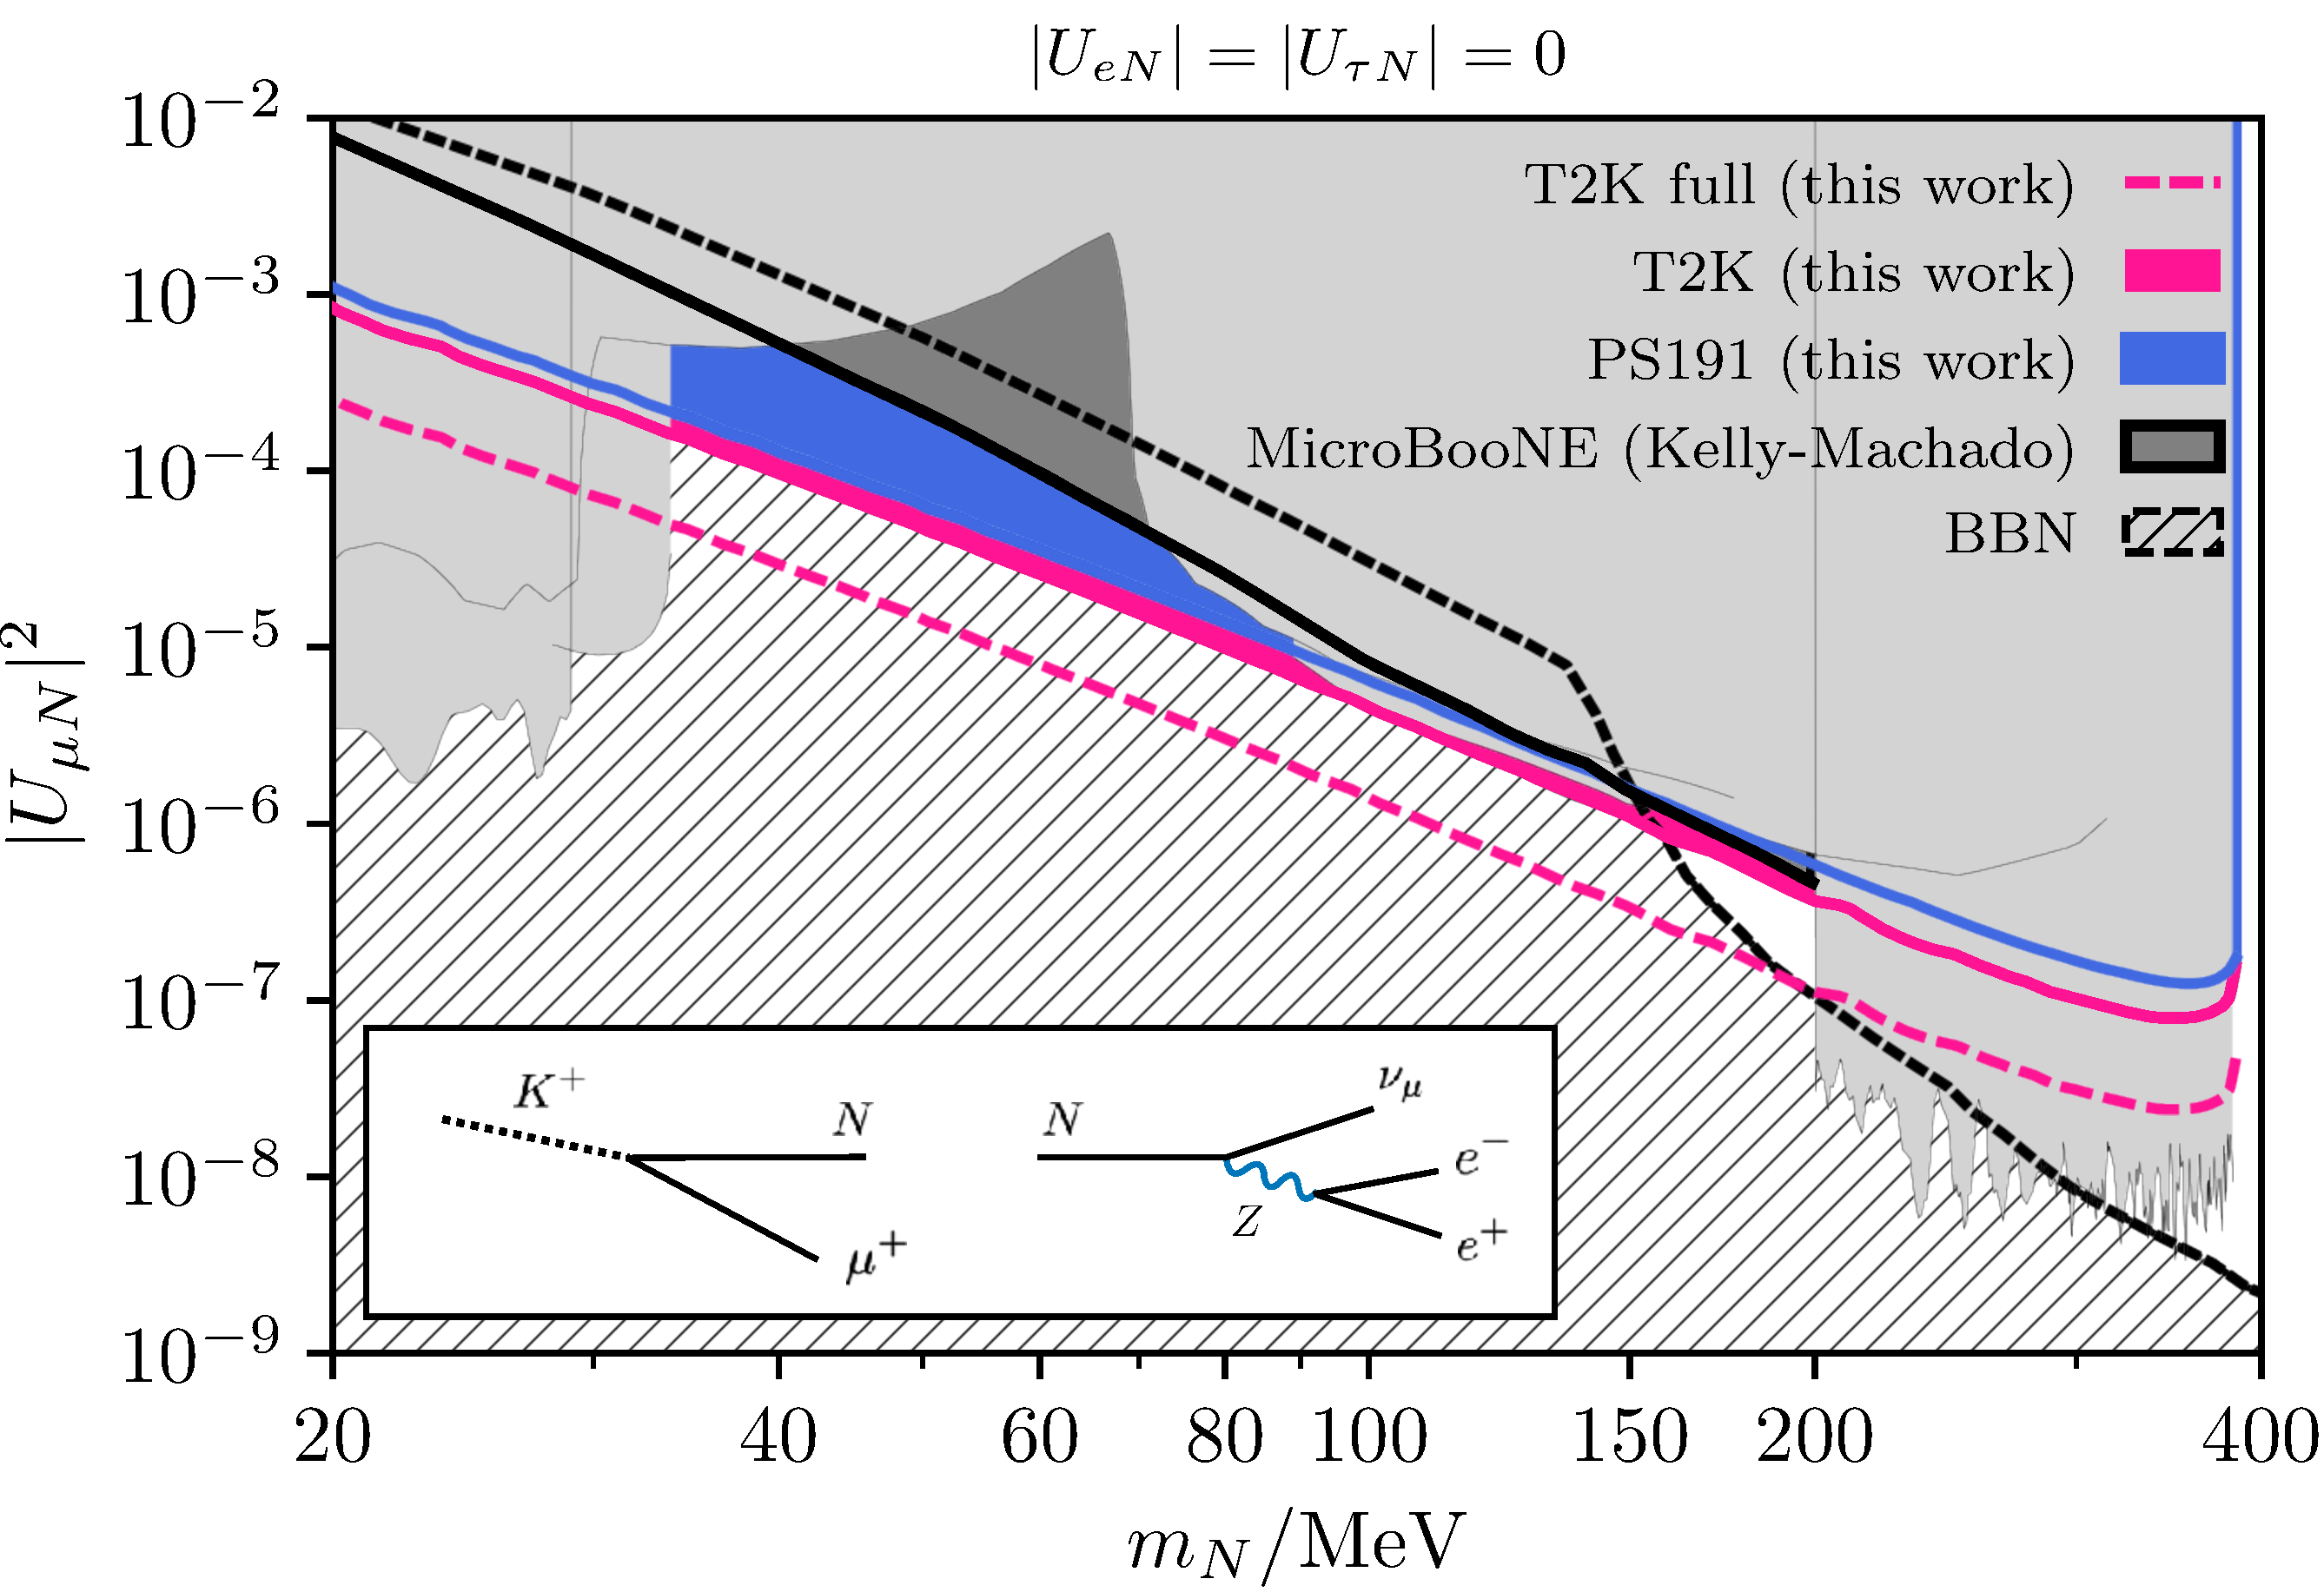
\includegraphics[width=\columnwidth]{figures/Fig-1.pdf}
    \caption{Constraints on the mixing of HNLs with the muon flavor as a function of its mass for a minimal HNL model at 90\% C.L. , considering only the production and decay mode: $K \rightarrow \nu_{\mu} N \rightarrow \nu_{\mu} (e^+e^-\bar{nu_{\mu}})$.
    For MicroBooNE, T2K, and PS191 the regions above the lines are excluded, while BBN excludes the region below the line. In gray we show other model-independent constraints.
    \label{fig:minimal}}
\end{figure}

At dimension six, we consider a vectorial four-lepton interaction
\begin{equation}\label{eq:dim-6}
    \mathcal{L} \supset \frac{G_X}{\sqrt{2}} \left(\overline{N} \gamma^\mu N \right) \left( \overline{\ell_\beta} \gamma_\mu \ell_\beta \right) + \text{h.c.},
\end{equation}
where $\beta \in \{e,\mu,\tau\}$. 
For $G_F/G_X \ll 1$, HNLs decay primarily via $N \to \nu \ell_\beta^+ \ell_\beta^-$ through mixing. 
Interesting completions of \cref{eq:dim-6} include gauged $U(1)_{B-L}$ extensions and dark $U(1)_X$ gauge symmetries~\cite{Bertuzzo:2018ftf,Abdullahi:2020nyr}.
In this latter model, the dark photon $A^\prime$ couples to dark leptons, $g_X \overline{N_D} \slashed{A}^\prime N_D$, and to charged SM particles via kinetic mixing with the photon, $(\varepsilon/2) F_{\mu\nu} X^{\mu\nu}$. 
Thus \cref{eq:dim-6} is independent of flavor, resulting in $G_X/\sqrt{2} \sim (g_X e \varepsilon)/m_{A^\prime}^2$, where $g_X$ is the gauge coupling. 
As a result, the amplitude for $N\to\nu e^+e^-$ is proportional to $G_X U_{\mu N}$, shortening the HNL lifetime by a factor $ \kappa \sim (G_F/G_X)^2$ with respect to the minimal model.
Model independent limits on kinetic mixing constrain $\kappa \gtrsim 10^{-4}$. 
%In addition, for theoretical consistency, such hidden sectors typically contain several HNLs, which may also be produced in the decay of their heavier partners. 
%Even faster decays like $N\to N^\prime \ell^+ \ell^-$ could dominate since the rate would be independent of $|U_{\mu N}|^2$. 
%We do not comment further on this possibility, and assume that decay rates mediated by \cref{eq:dim-6} are always proportional to $|U_{\mu N}|^2$.

% \begin{figure}[t]
%     \centering
%     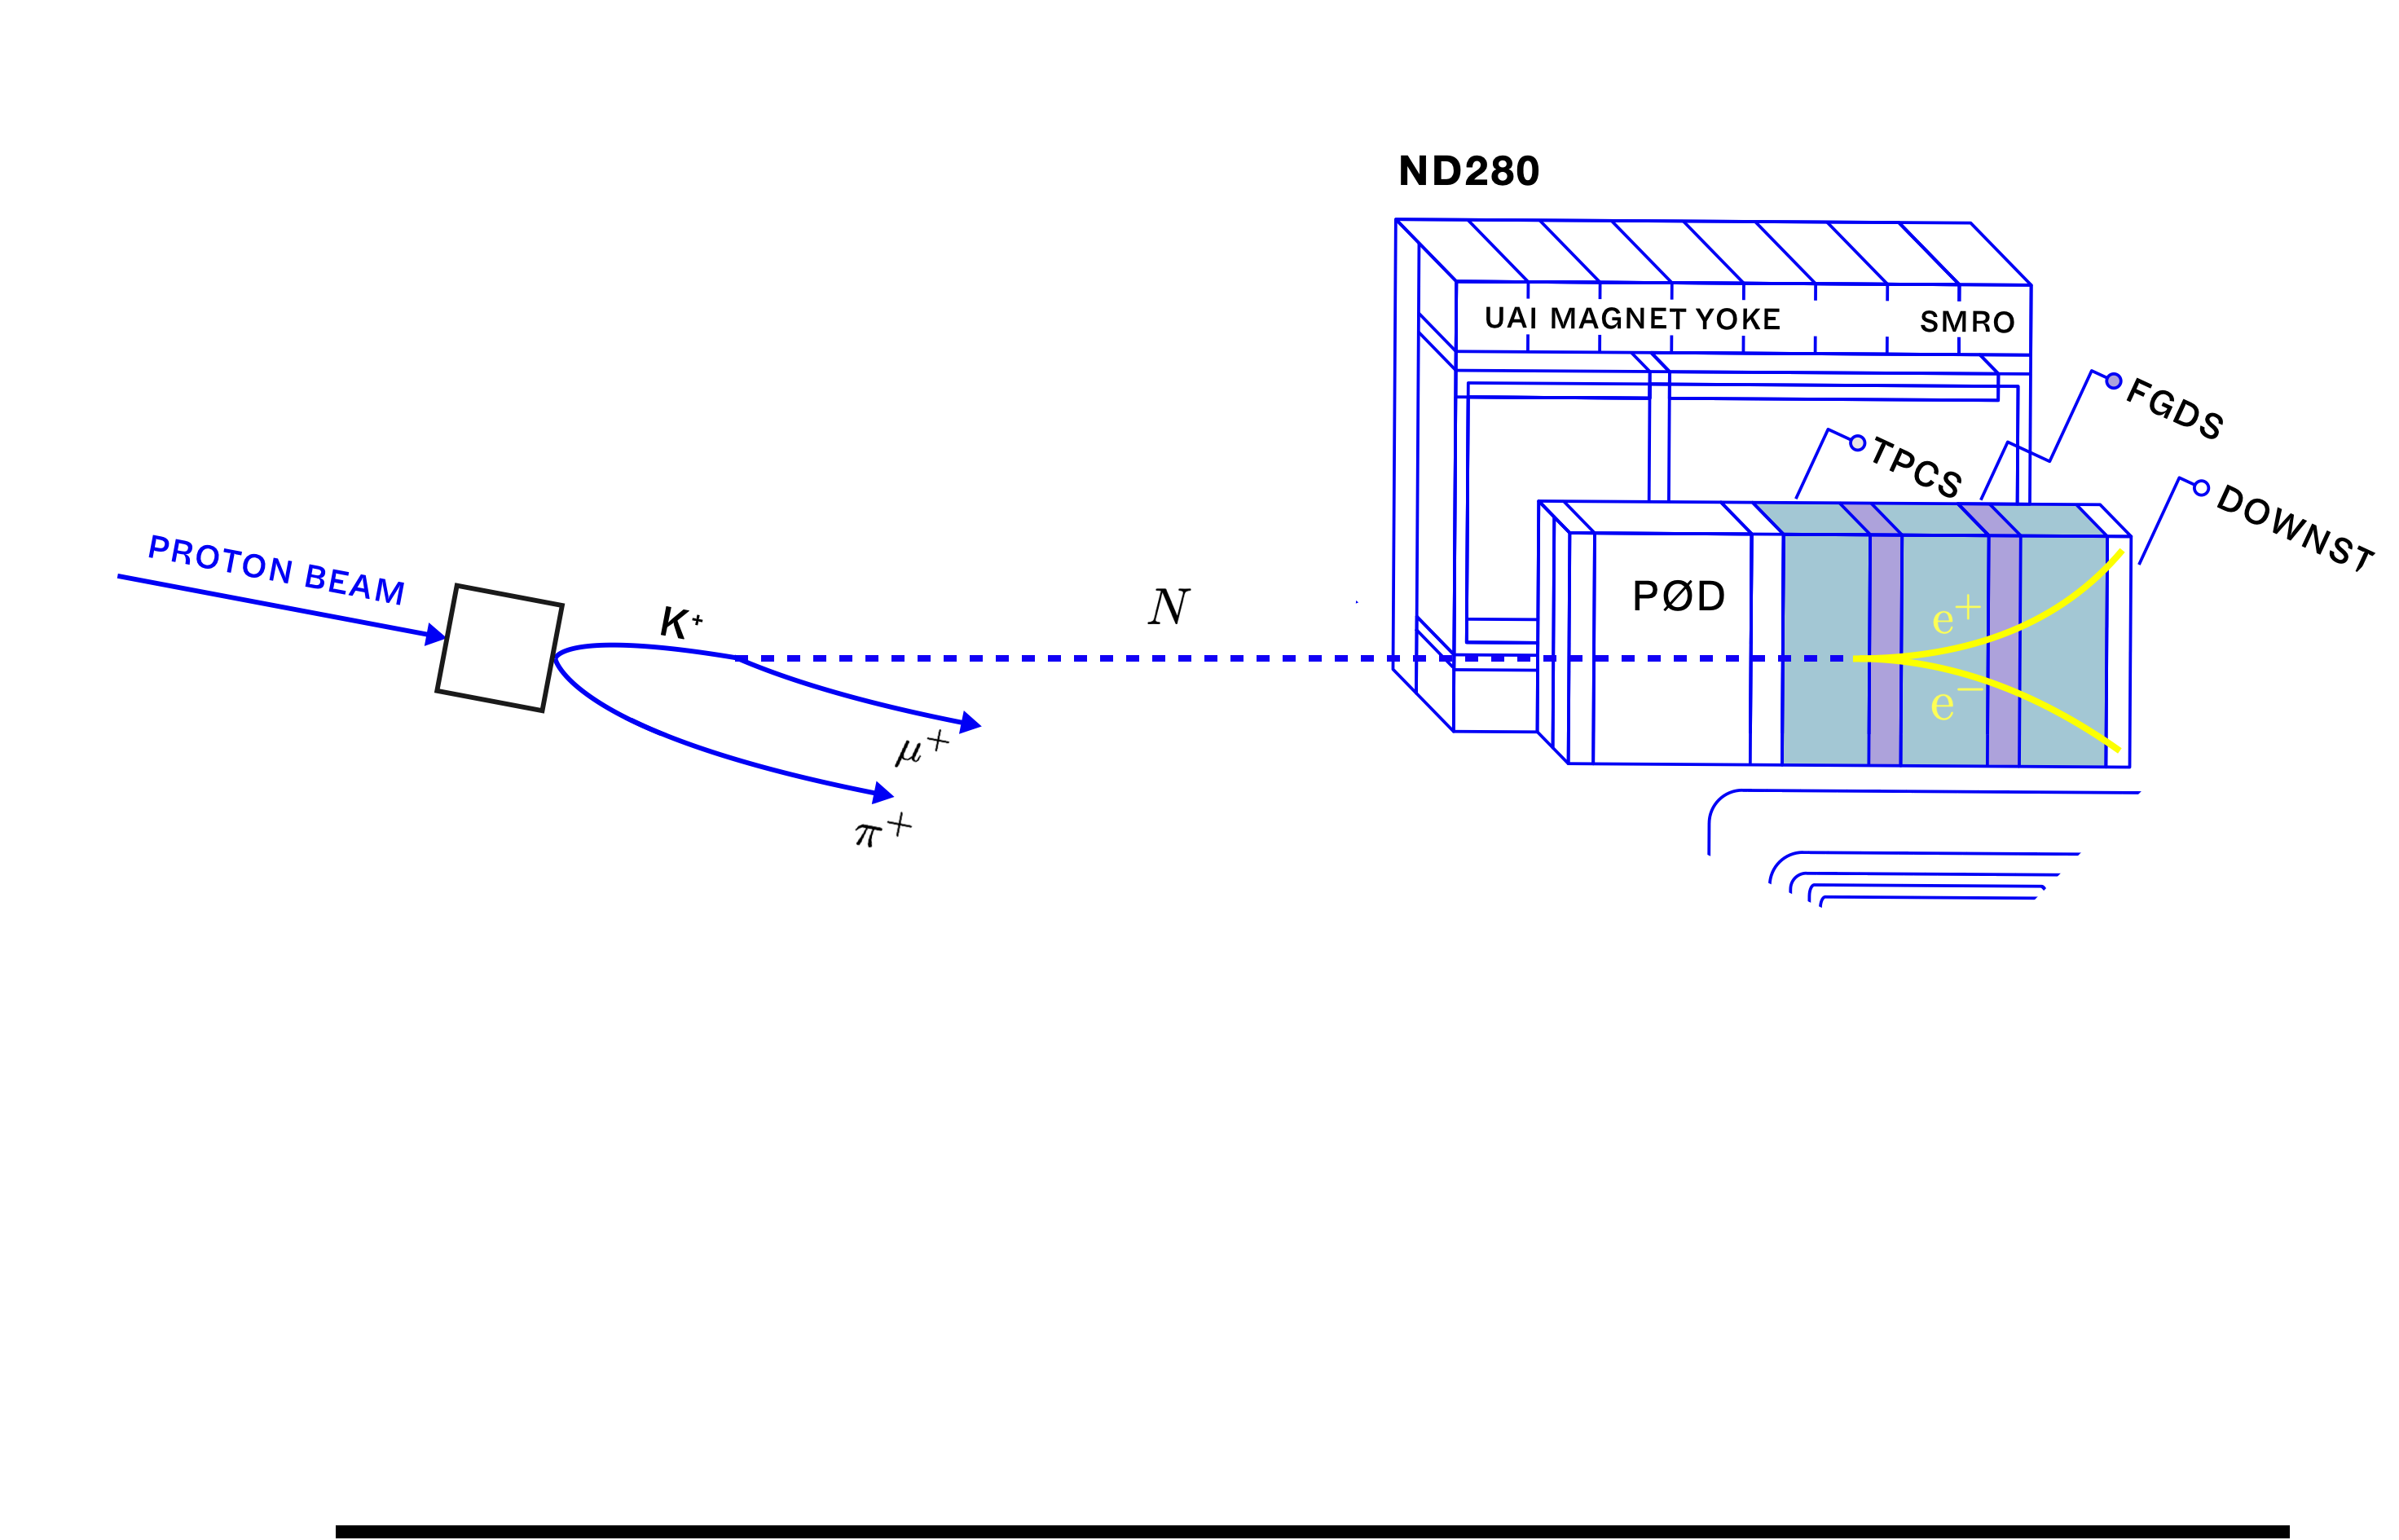
\includegraphics[width=\columnwidth]{new.png}
%     \caption{The T2K near detector, ND280, and the heavy neutrino decay-in-flight signature. The detector is located at an angle of $2.042^\circ$ with respect to the proton beam and at a distance of 284.9~m from the center of the production target.label{fig:diagram}}
% \end{figure}

\emph{HNLs at neutrino experiments.---}Accelerator neutrino beams are obtained from the DIF of magnetically-focused mesons. 
If HNLs exist, they are part of the neutrino beam produced through mixing.
The flux of HNLs in a given experiment can be estimated from the known neutrino flux per parent meson, by re-scaling it by~\cite{Shrock:1980vy,Shrock:1980ct}
\begin{equation}
    \rho(a,b) = \frac{\Gamma_{M\to N \ell}}{\Gamma_{M\to \nu \ell}} = |U_{\ell 4}|^2 (a+b-(a-b)^2)\sqrt{\lambda(1,a,b)},
\end{equation}
where $M$ is the associated parent meson, $a=(m_\ell,m_M)^2$, $b=(m_N/m_K)^2$, and $\lambda$ is the K\"all\'en function. 
In this work, we include only the contribution from kaon decays, neglecting production from pions and muons.
This rescaling method is sufficient in the low HNL mass region where $m_N \lesssim  (m_M - m_\ell)/2$, and automatically takes into account the effect of the magnetic focusing at the production point and other geometrical effects.
For larger $m_N$ values, our approach underestimates the HNL flux and therefore yields conservative results.
Heavier HNLs are produced with lower transverse momentum with respect to parent particles than light neutrinos. 
They are therefore more collimated with the beam direction, increasing the angular acceptance of on-axis detectors to HNLs, particularly at low energies where light neutrinos would have otherwise larger angular spread.

When considering new forces that shorten the lifetime, while keeping $N$ long-lived enough to reach the detector, the probability for $N$ to decay to some final state $X$ inside the detector is independent of the total lifetime ($1/\Gamma)$, and proportional only to the partial decay width in the signal channel ($\Gamma_{N\to X}$) 
\begin{align}\label{eq:prob_decay}
    P_{N\to X} &= e^{-L \Gamma/\beta\gamma} (1- e^{-\ell_{\rm det} \Gamma/\beta\gamma }) \, \mathcal{B}(N\to X) 
    \\\nonumber 
    &\simeq \frac{\ell_{\rm det}}{\gamma\beta} \, \Gamma_{N\to X},
\end{align}
where $\ell_d$ is the length of the detector, $L$ the distance between the production and decay points, $\gamma\beta = p_N/m_N$, and $\mathcal{B}$ denotes the branching ratio. 
Ultimately, in the long-lifetime and single-flavor-dominance limits, the new upper bound is given by $|U_{\alpha N}^{\rm new}|^2  = |U_{\alpha N}|^4  \times \widehat{\Gamma}_{N\to X} / \Gamma_{N\to X}^{\rm new}$, where $\widehat{\Gamma} = \Gamma/|U_{\alpha N}|^2$. 
The argument is analogous when relaxing the assumption of single-flavor dominance. 
If $\Gamma_{N\to X}^{\rm new} \propto |U_{\alpha N}^{\rm new}|^2$, the new upper-bound is proportional to the square-root of the ratio of signal decay rates, while the new lower bound, if it exists, will be linearly dependent on the ratio of the total rates. 
This is also approximately true for the lower bounds posed by cosmology.

\emph{T2K ND280.---}The T2K collaboration searched for the DIF of HNLs in the three Gaseous Argon Time Projection Chambers (GArTPC) of the off-axis near detector ND280~\cite{Abe:2019kgx}.
Because of the low density of the argon gas, this search has very small backgrounds from neutrino interactions, while the gas allows excellent tracking and identification of the $e^+e^-$ final state.
The analysis observes no event in all analysis channels, and provides some of the strongest limits in the mass region $\SI{140} \leq ~ m_N \leq \SI{493}\MeV$.
We use their null results and extrapolate the experimental efficiencies to estimate the constraint on light HNLs with $\SI{20} \leq ~ m_N \leq \SI{140} \MeV$.
We neglect systematic uncertainties and backgrounds, as they provide negligible contributions to the limits.
We reproduce the official T2K result above the pion mass with reasonable accuracy.

ND280 is currently being upgraded to a new configuration~\cite{T2K:2019bbb}, with the replacement of the $\pi^0$ detector, currently made of lead and scintillator, with two new GArTPCs.
DIF searches will benefit from the larger GAr volume and from the reduced number of backgrounds from coherent neutrino interactions upstream of the TPCs.
% A new time-of-flight detector will also be installed, which will reduce backgrounds from out-of-fiducial-volume interactions.
We estimate the sensitivity of a future search with this upgrade by considering the increased volume, and a total of $2\times 10^{22}$ POT~\cite{Abe:2016tii}, $4\times 10^{21}$ before (already collected), and $16\times 10^{21}$ after the upgrade.
This is a conservative estimate that neglects improvements to reconstruction and background rejection.
\begin{figure}[t]
    \centering
    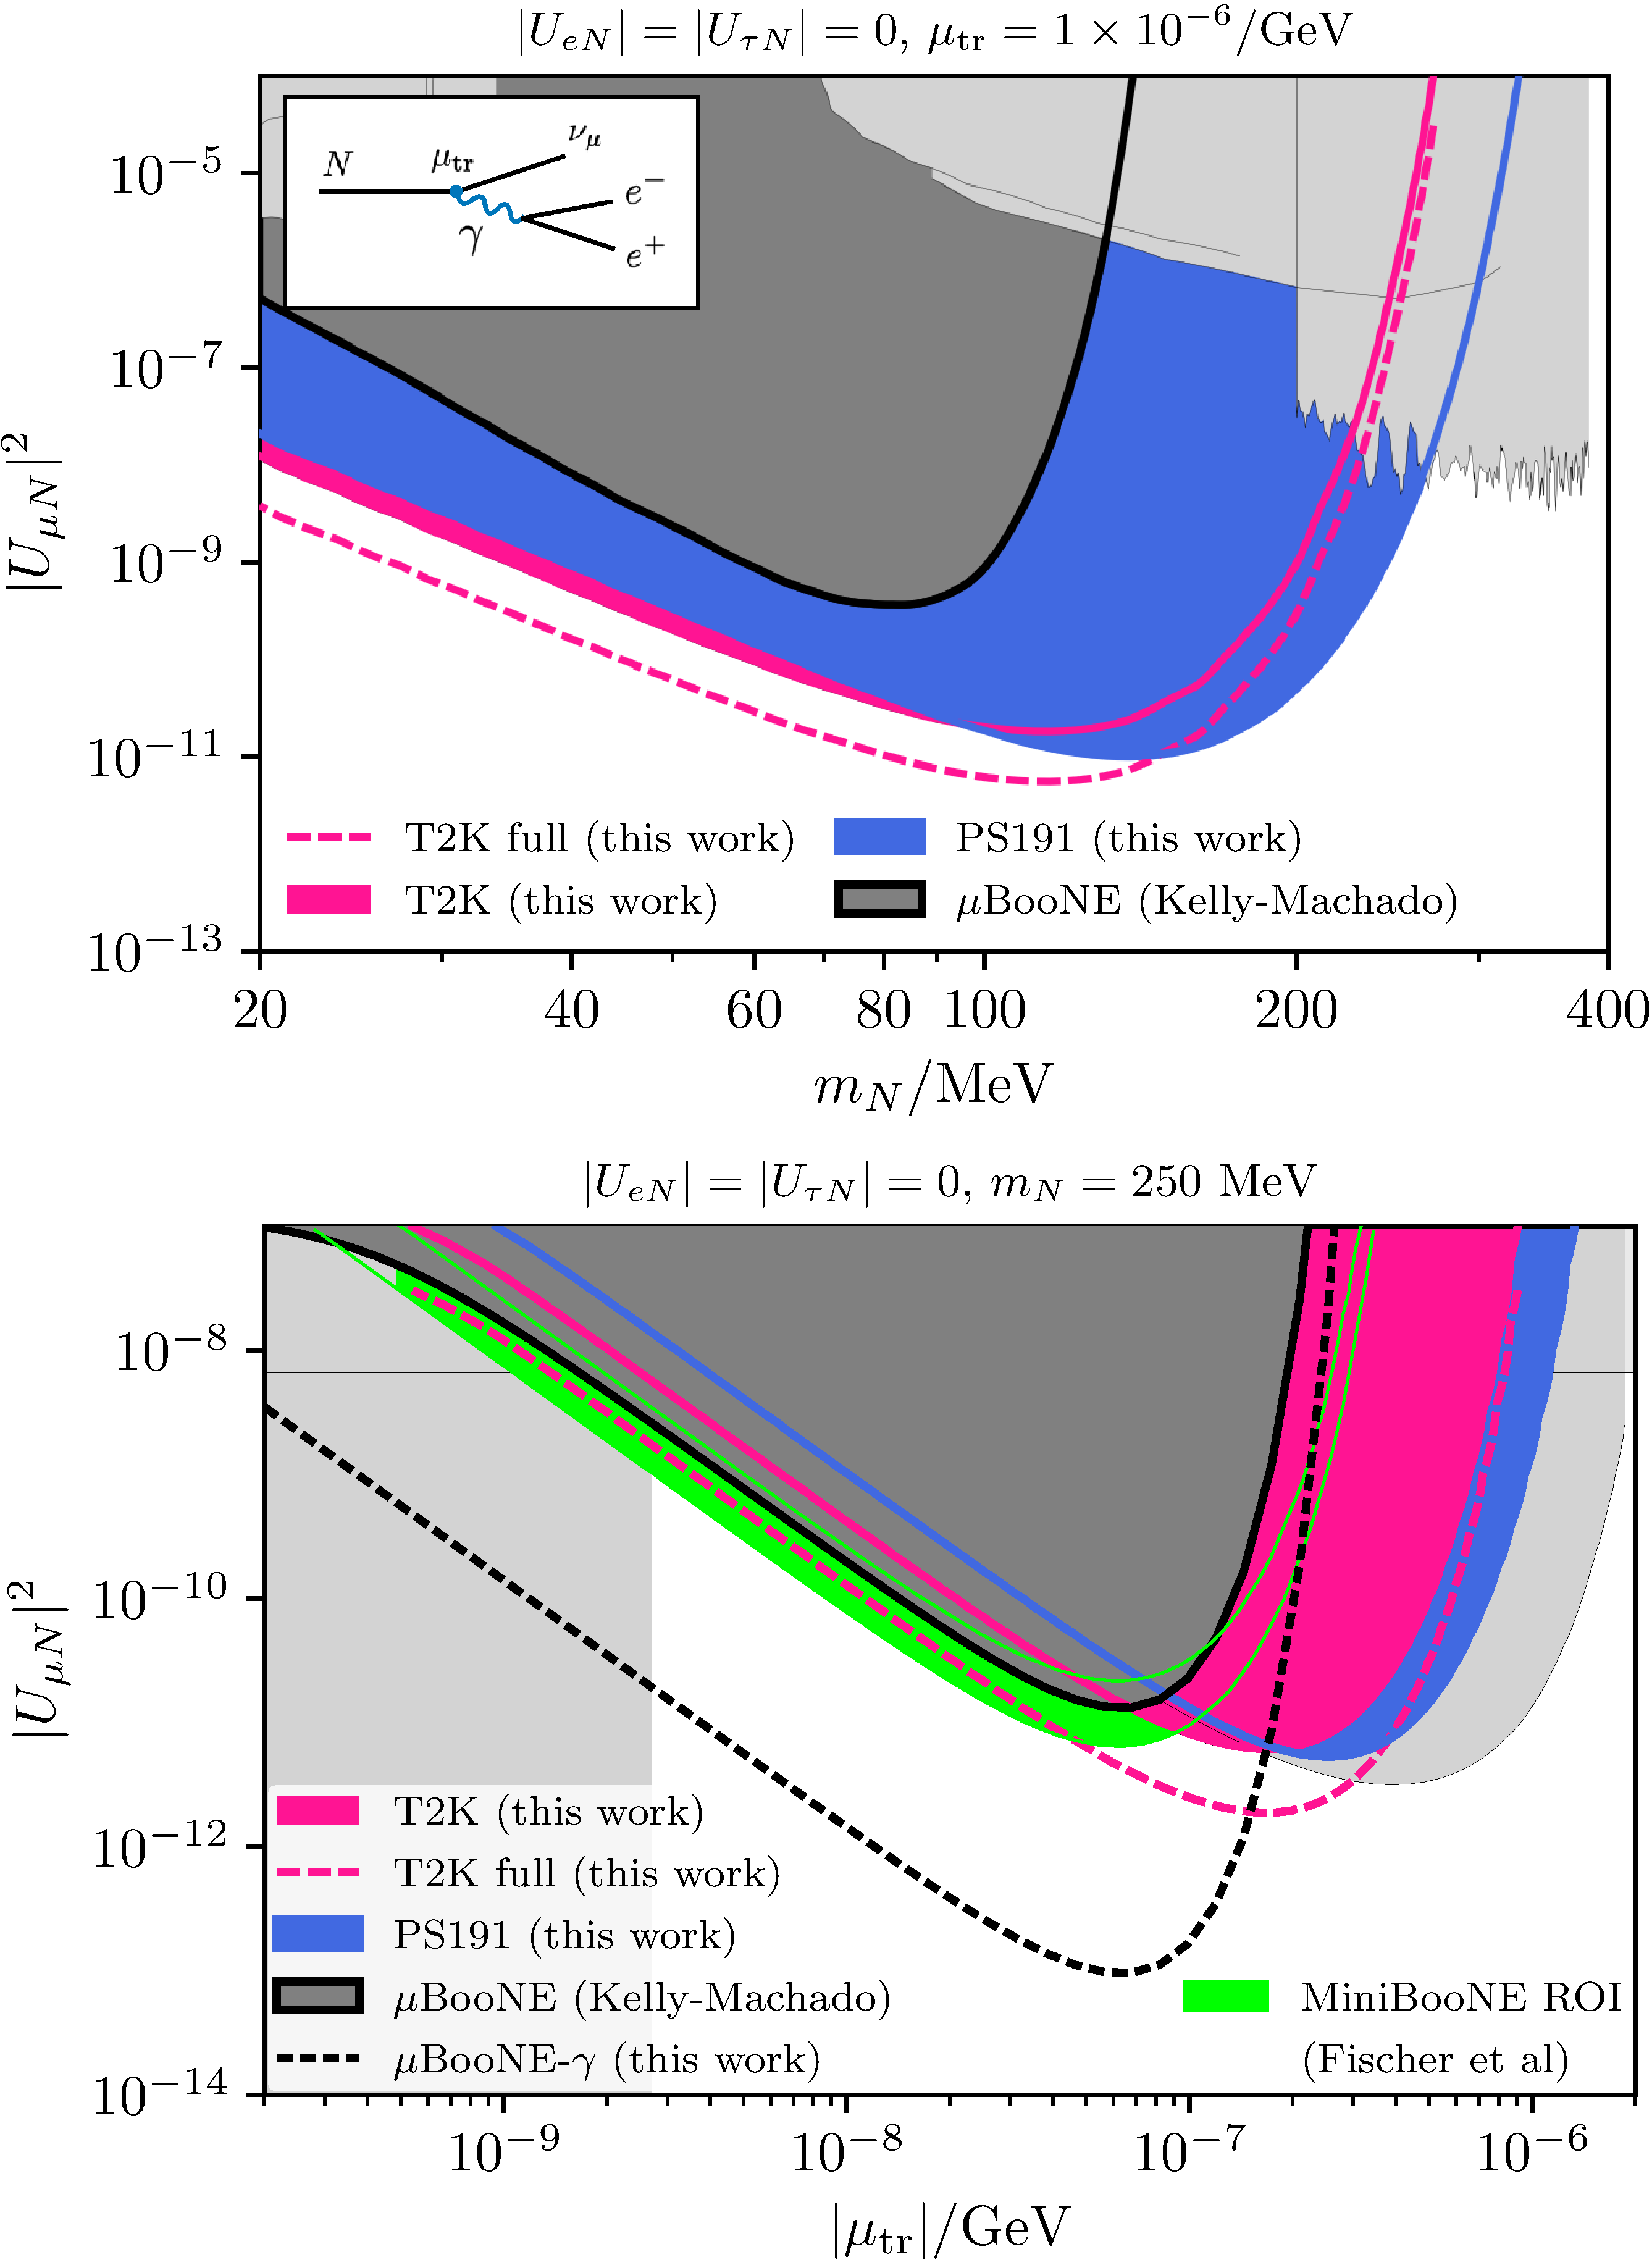
\includegraphics[width=\columnwidth]{figures/Fig-2.pdf}
    \caption{Top: Same as \cref{fig:minimal} but for HNLs with a TMM $\mu_{tr} = 1 \,\text{PeV}^{-1}$.
    Bottom: The same constraints as above but shown as a function of $\mu_{tr}$ for a fixed value of the HNL mass. The region of interest to explain the MiniBooNE excess is shown in green~\cite{Fischer:2019fbw}. In fine dashed black we show an optimistic estimate of a NuMI single-photon search at MicroBooNE.
    }
    \label{fig:dipole}
\end{figure}

\emph{MicroBooNE.---}MicroBooNE is the first ton-scale liquid argon (LAr) TPC operated in a neutrino beam.
It can perform searches for the DIF of new particles~\cite{Batell:2009di,Ballett:2016opr,Batell:2019nwo}.
However, since LAr is a high-density material, providing both the target and the detector material, one needs to rely on extra schemes to reject neutrino-induced background.
The delayed arrival of HNLs with respect to neutrinos 
was explored in the search for HNLs in the $\mu\pi$ decay channel~\cite{microboone_hnl}.
The authors of~\cite{Kelly:2021xbv} recast the null result of the MicroBooNE~\cite{MicroBooNE:2021ewq} search for light scalars into limits on the HNL mixing. 
This search successfully rejects background utilizing the directionality and time of arrival of new particles, as produced in decays at rest of kaons at the beam dump of the NuMI beam.
We further re-interpret this constraint as bounds on the non-minimal models considered.

\emph{PS191.---}PS191 was a low-density detector located at CERN and designed to search for the decays of long-lived particles. 
The 19.2~GeV proton beam provided a neutrino beam for the on-axis BEBC experiment, and could also be used by PS191 at 40~mrad off-axis location, where $\langle E_\nu \rangle\sim 1$~GeV.
The detector comprised of helium bags separated by scintillator planes followed by a dense electromagnetic calorimeter downstream~\footnote{The calorimeter was used in a search for $\nu_\mu \to \nu_e$ oscillations, where an excess was observed~\cite{Bernardi:1986hs}.}. 
Their final results considered only the CC decays of Dirac HNLs~\cite{Levy:1986yx,Bernardi:1987ek}.
% ~\footnote{In the first publication~\cite{Bernardi:1985ny} it was incorrectly stated that the limits are independent of the Dirac or Majorana nature of the HNLs, which was later corrected in~\refrefs{Levy:1986yx}{Bernardi:1987ek}.}. 
As a consequence, the search for $K^+\to\mu^+ (N \to \pi^+\mu^-)$ and $K^+\to \mu^+ (N\to \nu_e \mu^- e^+)$ was used to constrain only the $|U_{\mu N}|^2$-dominant case~\footnote{We note that the channel $K^+ \to \mu^+ (N \to \nu_\mu \mu^+ \mu^-)$ was not considered even though it also proceeds via CC diagrams and could also constrain $|U_{\mu N}|^2$.} and the search $K^+\to\mu^+ (N \to e^+e^-)$ was used to constrain $|U_{\mu N} U_{e N}|$. 
We are concerned with the latter case, as even in a $|U_{\mu N}|^2$-dominant case, HNLs still decay to $\nu e^+e^-$ via NC and a constraint can be derived. 
This point was first appreciated in~\cite{Kusenko:2004qc} and later discussed in~\cite{Ruchayskiy:2011aa,Drewes:2015iva}. 
These constraints were thought to be the strongest lab-based ones in this mass region for the $|U_{\mu N}|^2$-dominant case. 
With our simulation, we show that this is not the case.
The bound on $|U_{\mu N}|^2$ is a factor of 6 weaker than the published ones, corresponding to an event rate 36 times smaller~\footnote{We have found a similar factor in the channels $N\to \mu \pi$ and $N\to \nu e \mu$. For the latter, we find a discrepancy by a factor of 6 at the largest HNL masses, which decreases for lower HNL masses. We attribute this effect to us overestimating the signal efficiency. For $\mu\pi$, the discrepancy is a constant factor of 7.5.}. 
This is corroborated by the fact that T2K and PS191 have very similar total exposures and neutrino fluxes, noting that PS191 ran for only a month.

If constraints on light scalars can be translated to constraints on HNLs, as illustrated in~\cite{Kelly:2021xbv}, it follows that the converse is also true. For example, \cite{Gorbunov:2021ccu} used the null results from PS191 to cast limits on the light scalar $\phi$. 
For the muon-dominant case, this is a trivial translation, as $K\to \pi \phi$ and $K\to \mu N$ have very similar kinematics. 
Our new PS191 limits recasted for scalars agree with~\cite{Gorbunov:2021ccu}. 
We also note that eecasting our results below for current (future) T2K data, we find a constraint on the scalar mixing of $\theta< 2.3 \, (1.5) \times 10^{-4}$ for $m_\phi = 150$~MeV, which is the leading constraint in the ``pion gap''~\cite{Fuyuto:2014cya}.

\begin{figure}[t]
    \centering
    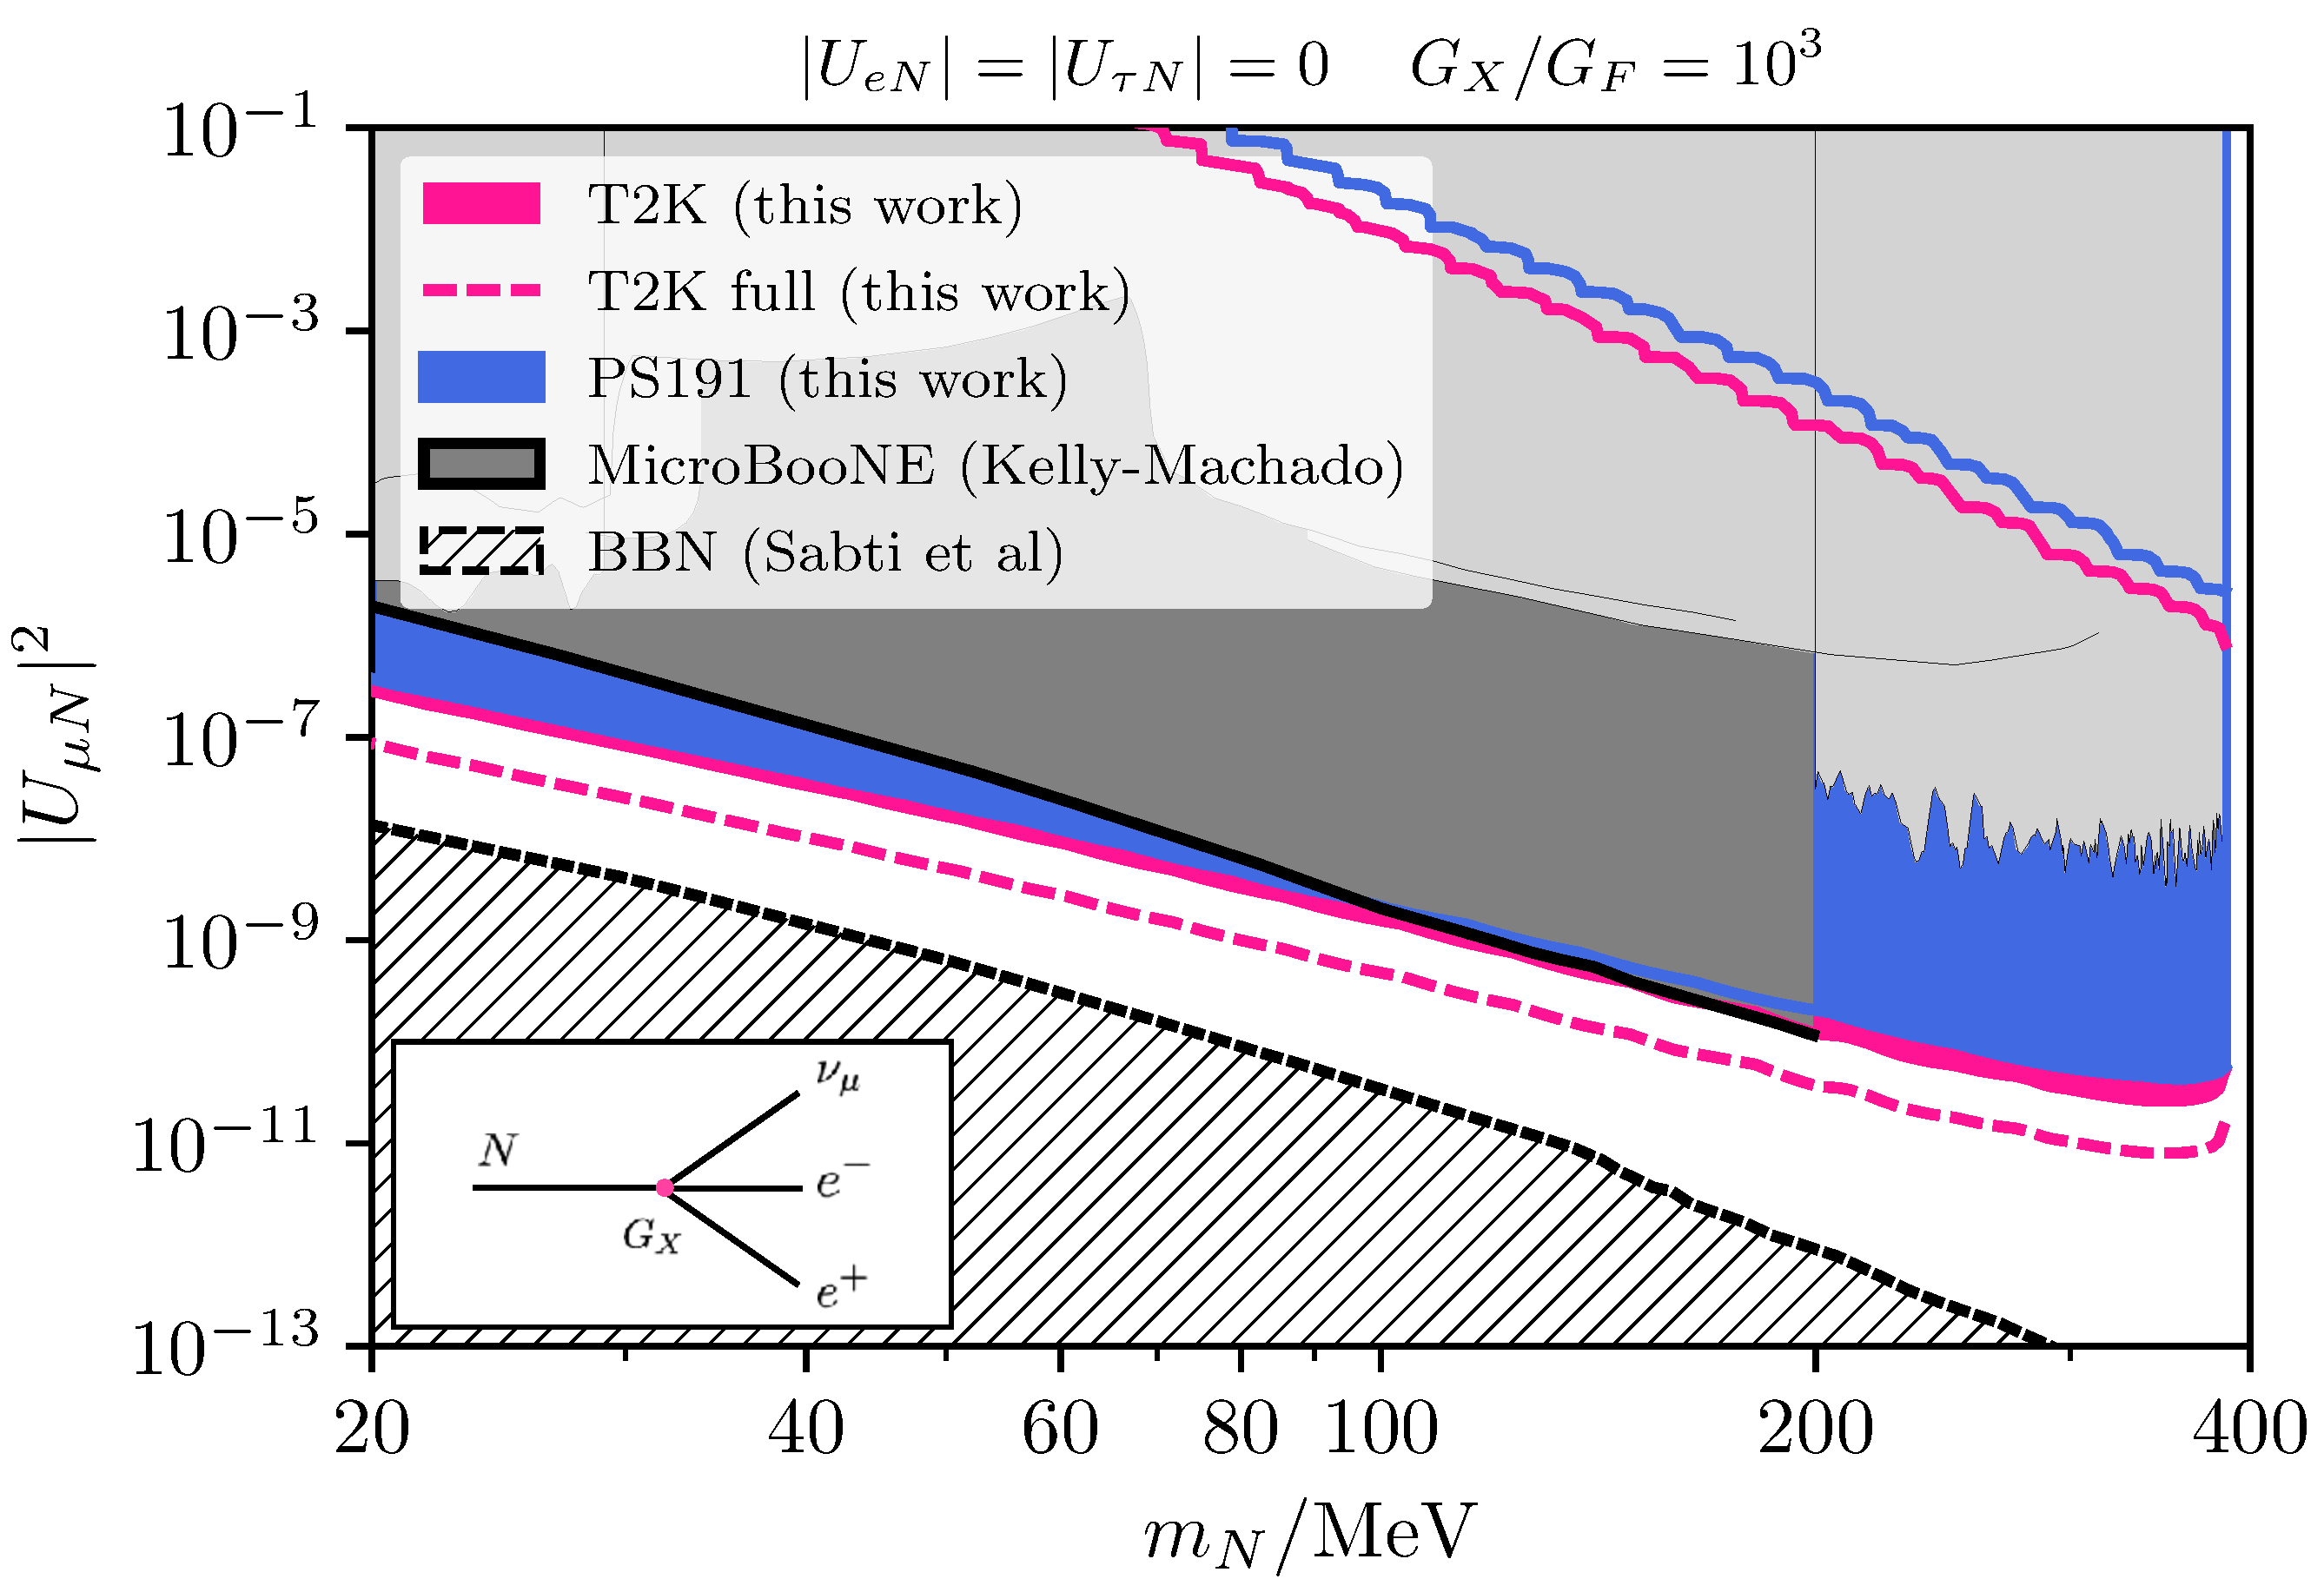
\includegraphics[width=\columnwidth]{figures/Fig-3.pdf}
    \caption{Same as \cref{fig:minimal} but for HNLs with a four-fermion leptonic interaction with $G_X = 10^{3} G_F$.}
    \label{fig:hidden_sector}
\end{figure}

\emph{Results and discussion.---}Our results for the minimal model are shown in \cref{fig:minimal}. 
Our bounds and sensitivity estimates rule out HNLs below the kaon mass with dominant muon mixing in the minimal model. 
This result also puts more strain on models that could also account for the baryon asymmetry of the Universe~\cite{Bondarenko:2021cpc}.
We have also shown that previous limits from PS191 have been overestimated by an order of magnitude, and that T2K provides the leading constraints at the lowest masses. 
Future data can improve the leading constraints below $\SI{200}\MeV$, where the kaon peak searches become insensitive.
We note that our results are based on extrapolated efficiencies and conservative flux simulation, and that a complete simulation within the collaboration will provide improved results.

The new constraints with decays via the dimension five, \cref{eq:dim-5}, are shown in \cref{fig:dipole}, while for dimension six, \cref{eq:dim-6}, in \cref{fig:hidden_sector}. 
In these scenarios the combination of lab-based and cosmological constraints do not exclude HNLs below the kaon mass.
Our work complements searches for neutrino upscattering at CHARM-II, which provides stronger constraints for new physics scales below $\SI{1}\PeV$~\cite{Coloma:2017ppo,Magill:2018jla}, and constraints from supernova, which dominate above $\sim\SI{1}\EeV$.
For $G_X/G_F=10^{3}$, BBN constraints still exclude the smallest mixings, but our lab-based results provide the best upper limits in the newly allowed parameter space. 
For this choice of parameters, one expects the existence of a new vector mediator with a mass of a few GeV, which can be searched for in collider experiments~\cite{Fabbrichesi:2020wbt}.

We now comment on the kinematics of HNL decays. 
Decays via NC or CC do not differ significantly in regards to the experimental variables upon which the signal efficiency depends.
This remains true for both the Dirac and Majorana cases, as well as for the additional interactions in \cref{fig:dipole} and \cref{fig:hidden_sector}, rendering the constraints mostly independent of the specifics of the HNL interactions. 
The most distinct case is the TMM, where the final products have smaller opening angles and are less collimated with the beam.
Nevertheless, in most events the physical separation between the electrons remains large, especially with magnetic fields. 
The impact of the new interactions on the selection efficiency should be studied by the T2K collaboration with its full detector simulation, but we do not expect significant changes to our results.

Our constraints are relevant to new physics explanations of the MiniBooNE excess of electron-like events~\cite{MiniBooNE:2018esg,MiniBooNE:2020pnu}. 
The authors of~\cite{Fischer:2019fbw} proposed that the excess can be explained by the DIF of HNLs with a TMM. 
This observation can be generalized to any model with enhanced $N\to \nu e^+e^-$ or $\nu \gamma$ rates. 
The MiniBooNE region of interest and our constraints in~\cref{fig:dipole}, show that MicroBooNE and T2K are already constraining interesting parameter space for the TMM model.
Future T2K data will shine further light on this interpretation.

We also draw a sensitivity estimate of a search for single photons with the same efficiencies, backgrounds, and exposure as the $e^+e^-$ search at MicroBooNE, which could completely test the MiniBooNE excess in this model. 
This complementary strategy can only be achieved in high-density detectors, but is limited by the neutrino-induced backgrounds.  
With a volume of 0.66 and 4.5 times the \muboone~volume, respectively, and a similar beam exposure, SBND~\cite{sbnd} and ICARUS~\cite{icarus} could complement the MicroBooNE constraints, thanks to the different distances from beam target and absorber.

When the HNLs are too short-lived to be probed in DIF searches, they may be produced by coherent neutrino-nucleus upscattering in the dense lead layers of ND280~\cite{Gninenko:2009ks,Gninenko:2010pr,Coloma:2017ppo,Vergani:2021tgc,Bertuzzo:2018itn,Ballett:2018ynz,Ballett:2019pyw}.
A detailed study of this scenario is in progress~\cite{upcoming}. 
Prompt HNL decays in pion and kaon factories, such as PIENU~\cite{PIENU:2017wbj,PIENU:2019usb} and NA62~\cite{NA62:2021bji,NA62:2020mcv}, should also be searched for. 
The channel $K^+\to\ell^+ (N \to \nu e^+e^-)$, proposed in~\cite{Ballett:2019pyw}, would be sensitive to light dark sector models and, to a lesser extent, to TMM.

Our work shows that ND280 is one of the most sensitive experiments to long-lived particles.
Due to its hybrid design, ND280 can also place strong limits on upscattering production of light particles, like dark neutrinos~\cite{Bertuzzo:2018itn,Ballett:2018ynz,Ballett:2019pyw,upcoming} and co-annihilating dark matter~\cite{Tucker-Smith:2001myb,Izaguirre:2017bqb}.
Future detectors, such as the planned DUNE near detector, could also benefit from a hybrid detector design, since they would be sensitive to both charged-track and single photon final states, while having a region of low neutrino-induced backgrounds.

\acknowledgments
We acknowledge useful discussions with Kevin Kelly, Mathieu Lamoureux, Pedro Machado, Sophie King, and Teppei Katori.
C.A.A. is supported by the Faculty of Arts and Sciences of Harvard University, and the Alfred P. Sloan Foundation. 
N.F.’s work is supported by the Department of Energy grant award number DE-SC0007881.
The research of M.H. was supported in part by Perimeter Institute for Theoretical Physics. Research at Perimeter Institute is supported by the Government of Canada through the Department of Innovation, Science and Economic Development and by the Province of Ontario through the Ministry of Research, Innovation and Science. Part of M.H.'s work was performed at the Aspen Center for Physics, which is supported by National Science Foundation grant PHY-1607611.


\bibliographystyle{apsrev4-1}
\bibliography{lib}{}

\end{document}
